\chapter{State of the Art}
\label{SoA:estado del arte}

\section{Artificial Intelligence}
\label{Artificial Intelligence}
John McCarthy defines \gls{ai} as \enquote{The science and engineering of making intelligent machines, especially intelligent computer programs. It is related to the similar task of using computers to understand human intelligence, but AI does not have to confine itself to methods that are biologically observable}~\cite{aidefinitionjhon}. Other approaches such as the one used by Stuart Russel and Peter Norving~\cite{aiModern} organize all the definitions of \gls{ai} into four different categories depending on either \enquote{fidelity to human performance} or \enquote{ideal performance, called rationality}, as shown in Table~\ref{tab:groups-ai-def}.

\begin{table}[]
\caption{\label{tab:groups-ai-def}Definitions of AI organized according to Stuart Russel and Peter Norving}
\centering
\begin{tabular}{|c|c|}
\hline
\begin{tabular}[c]{@{}c@{}}\textbf{Thinking Humanly}\\ \\ The cognitive modeling approach\end{tabular} &
  \begin{tabular}[c]{@{}c@{}}\textbf{Thinking Rationality}\\ \\ The \enquote{laws of thought} approach\end{tabular} \\ \hline
\begin{tabular}[c]{@{}c@{}}\textbf{Acting Humanly}\\ \\ The Turing test approach\end{tabular} &
  \begin{tabular}[c]{@{}c@{}}\textbf{Acting Rationality}\\ \\ The rational agent approach\end{tabular} \\ \hline
\end{tabular}
\end{table}

The foundation and evolution of \gls{ai} is based on several fields of human knowledge which contributed ideas, viewpoints and techniques. Among those the following stand out:~\cite{aiState}

\begin{itemize}
    \item \textbf{Philosophy}: Brings up the idea of reasoning and understanding, laws governing the rational part of the mind, knowledge acquisition, the connections between knowledge and action and how conclusions can be drawn from formal rules.
    \item \textbf{Mathematics}: A certain level of mathematical formalization is needed to achieve a formal science. We can find three fundamental areas: probability, logic and computation.
    \item \textbf{Economics}: This science aims to study how to make choices that lead to preferred outcomes. \gls{dt} provides a formal framework for decisions made under uncertainty in the decision maker's environment, contributing to the concept of rational agent. 
    \item \textbf{Neuroscience}: How do brains process information? This raises the question of how intelligence and rationality function organically. Moreover, even though brains and digital computers have different properties, several neuroscience concepts have been applied to \gls{ai}, e.g. the abstraction of neurons used in deep learning algorithms. 
    \item \textbf{Psychology}: \gls{cs} gives the idea of how humans and animals think and act.
    \item \textbf{Computer engineering}: The computer is the artifact used for \gls{ai}. Due to the increase in performance and efficiency in each new generation of hardware and thanks to the software side of computer science, \gls{ai} has been able to evolve through out the years.
    \item \textbf{Control theory and cybernetics}: Norbet Wiener was the father of the \gls{ct}, which studies how artifacts can operate under their own control with feedback for adjusting to the environment.
    \item \textbf{Linguistics}: \gls{cl} or \gls{nlp} addresses the complex problem of understanding language and therefore the subject matter and context.
\end{itemize}

\notebox{
    \textbf{\enquote{Artificial Intelligence, A Modern Approach}}
    
    Written by Stuart Russel and Peter Norving, provides useful information about several introductory topics such as: extended definition, foundations of the field, background history and many more.
    I strongly recommend this reading for those seeking a deep insight into \gls{ai}.
}

\newpage

\subsection{Applications of Artificial Intelligence}

Figure~\ref{fig:state-art-ai} shows a carefully curated graph representing the evolution of \gls{ai} models classified by area and subarea~\cite{sotaAI} from which we can extract some current use cases of \gls{ai}. Specifically, we will focus on the following subareas:

\begin{figure}[H]
    \centering
    \caption{\label{fig:state-art-ai} Evolution of Models of AI}
    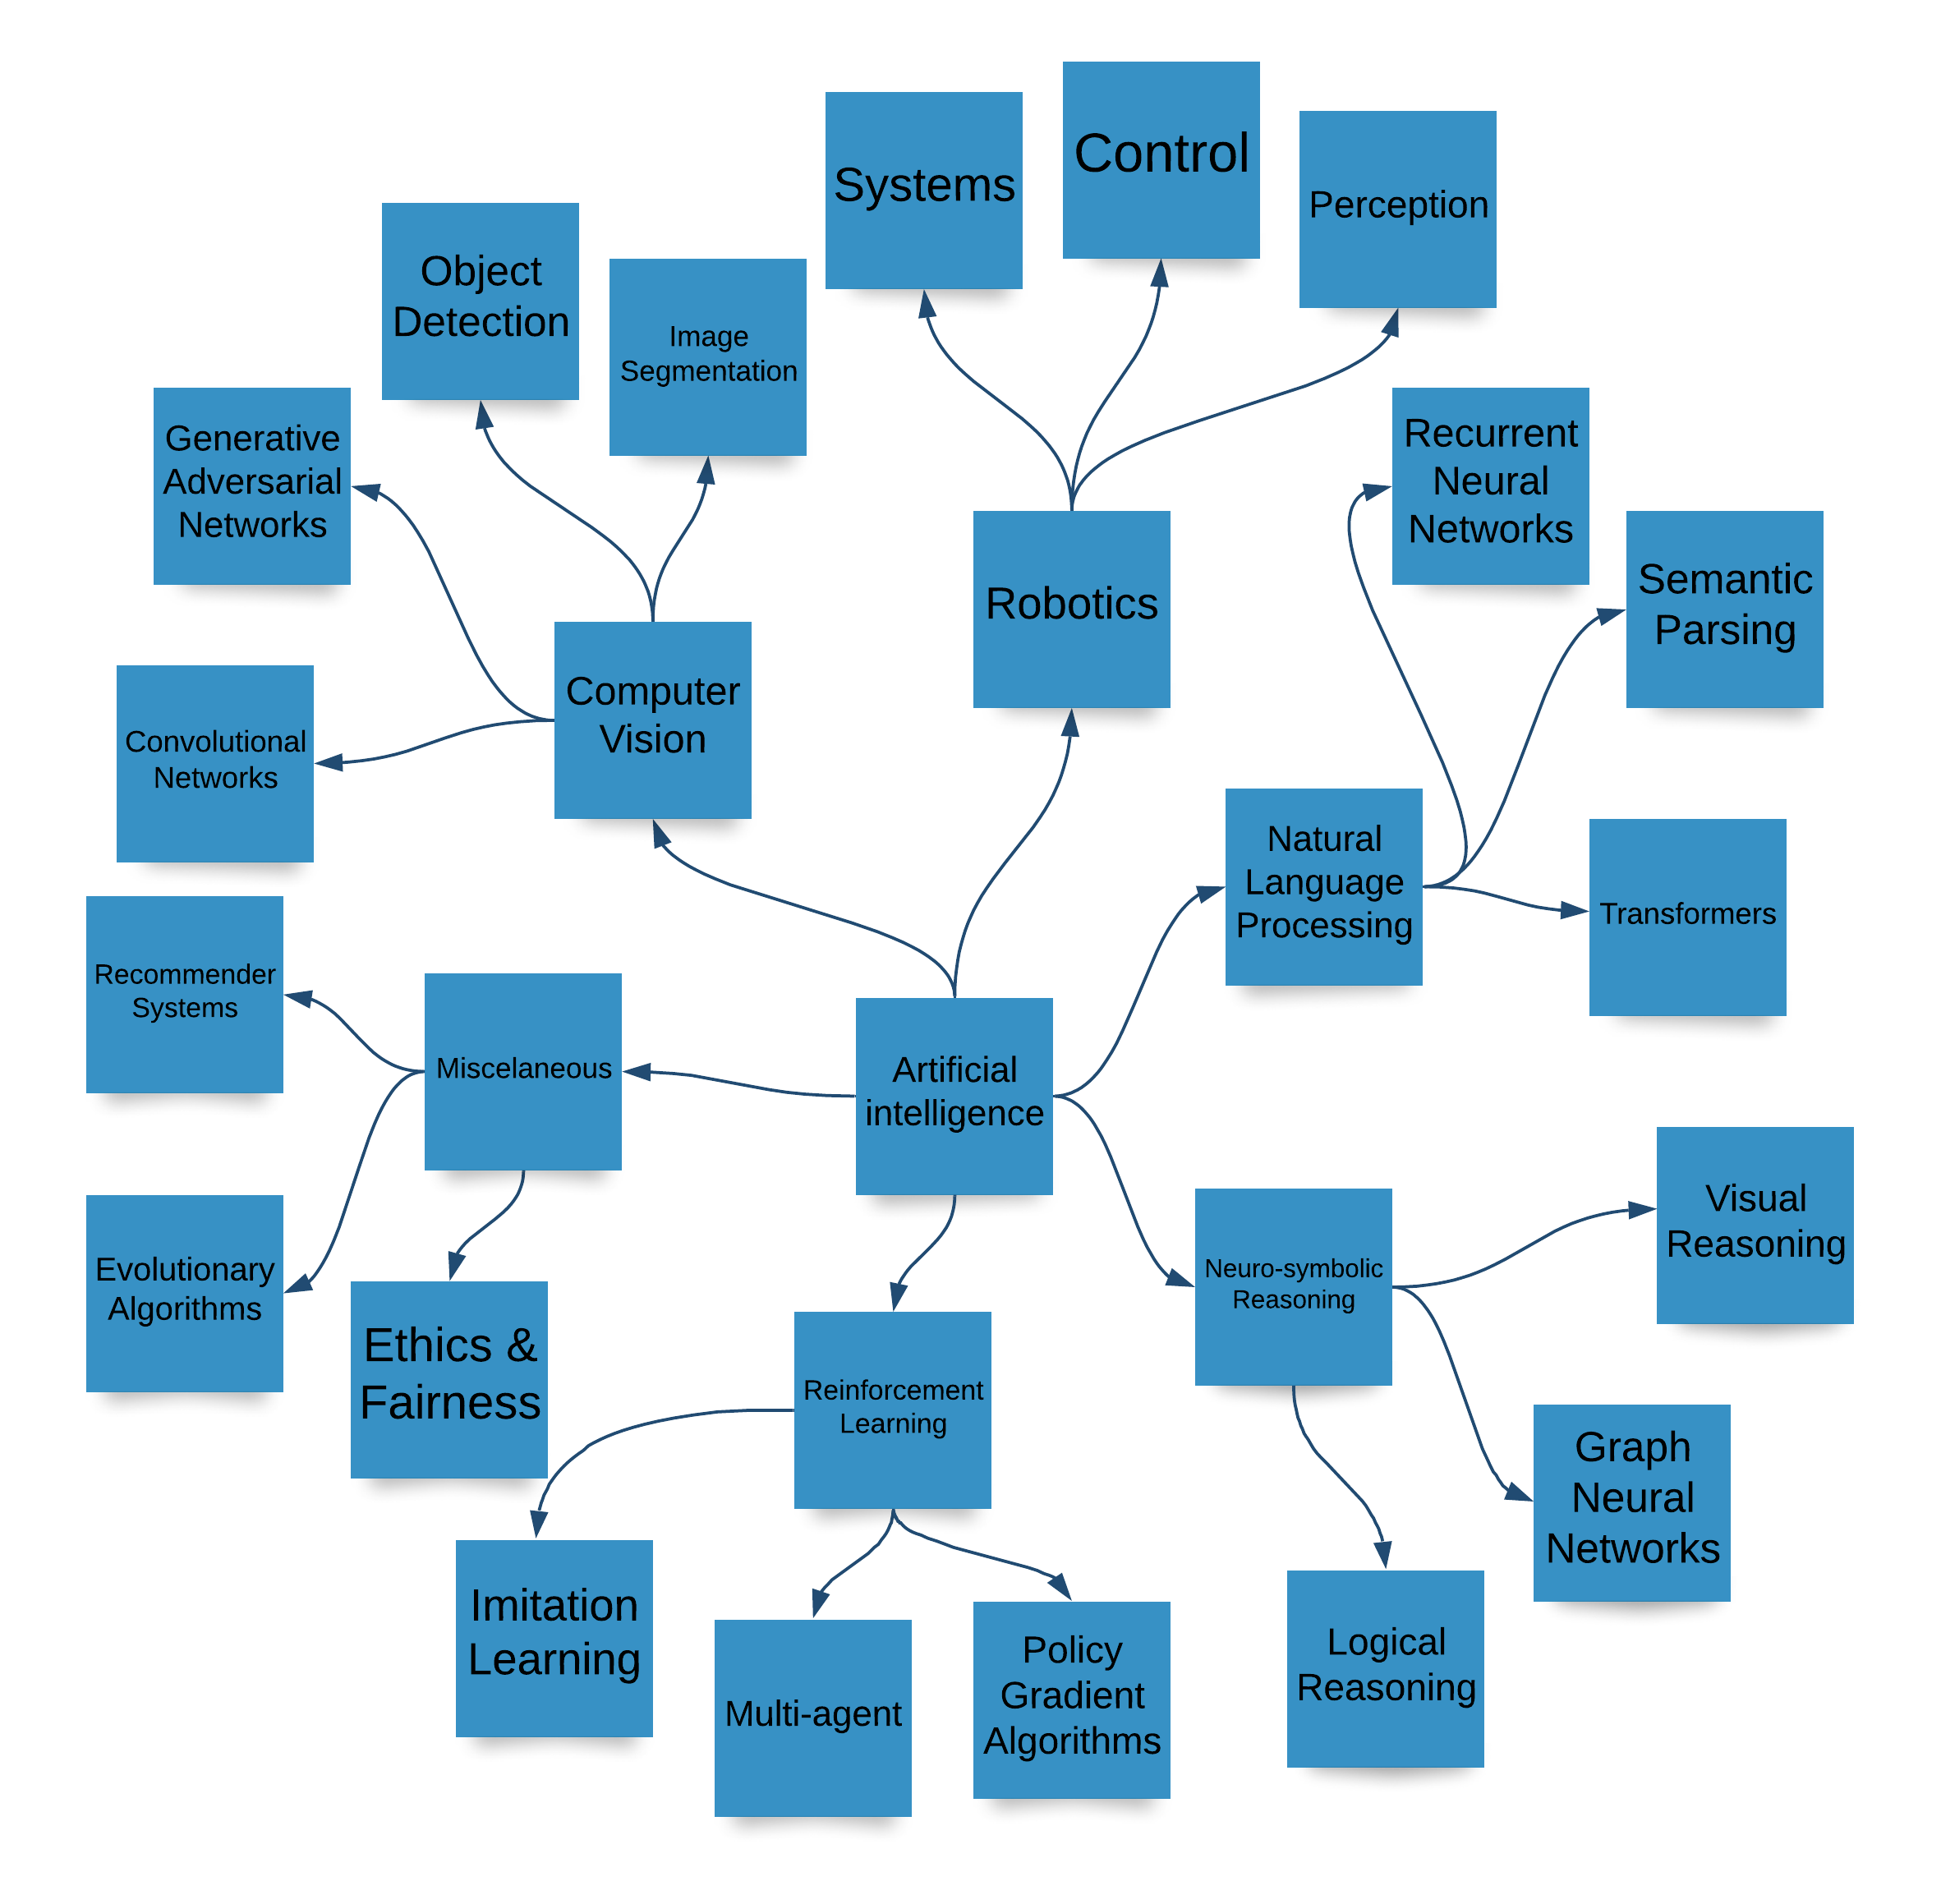
\includegraphics[width=0.85\textwidth]{figures/stoai.png}
\end{figure}

\newpage
\subsection{Deep Learning}

It is important to state the difference between the fields of \gls{ai} and \gls{dl}, since this thesis will focus mainly on the last one. 

\begin{wrapfigure}{l}{0.35\textwidth}
    \centering
    \caption{\label{fig:difference-ml-dl} Subfields Artificial Intelligence}
    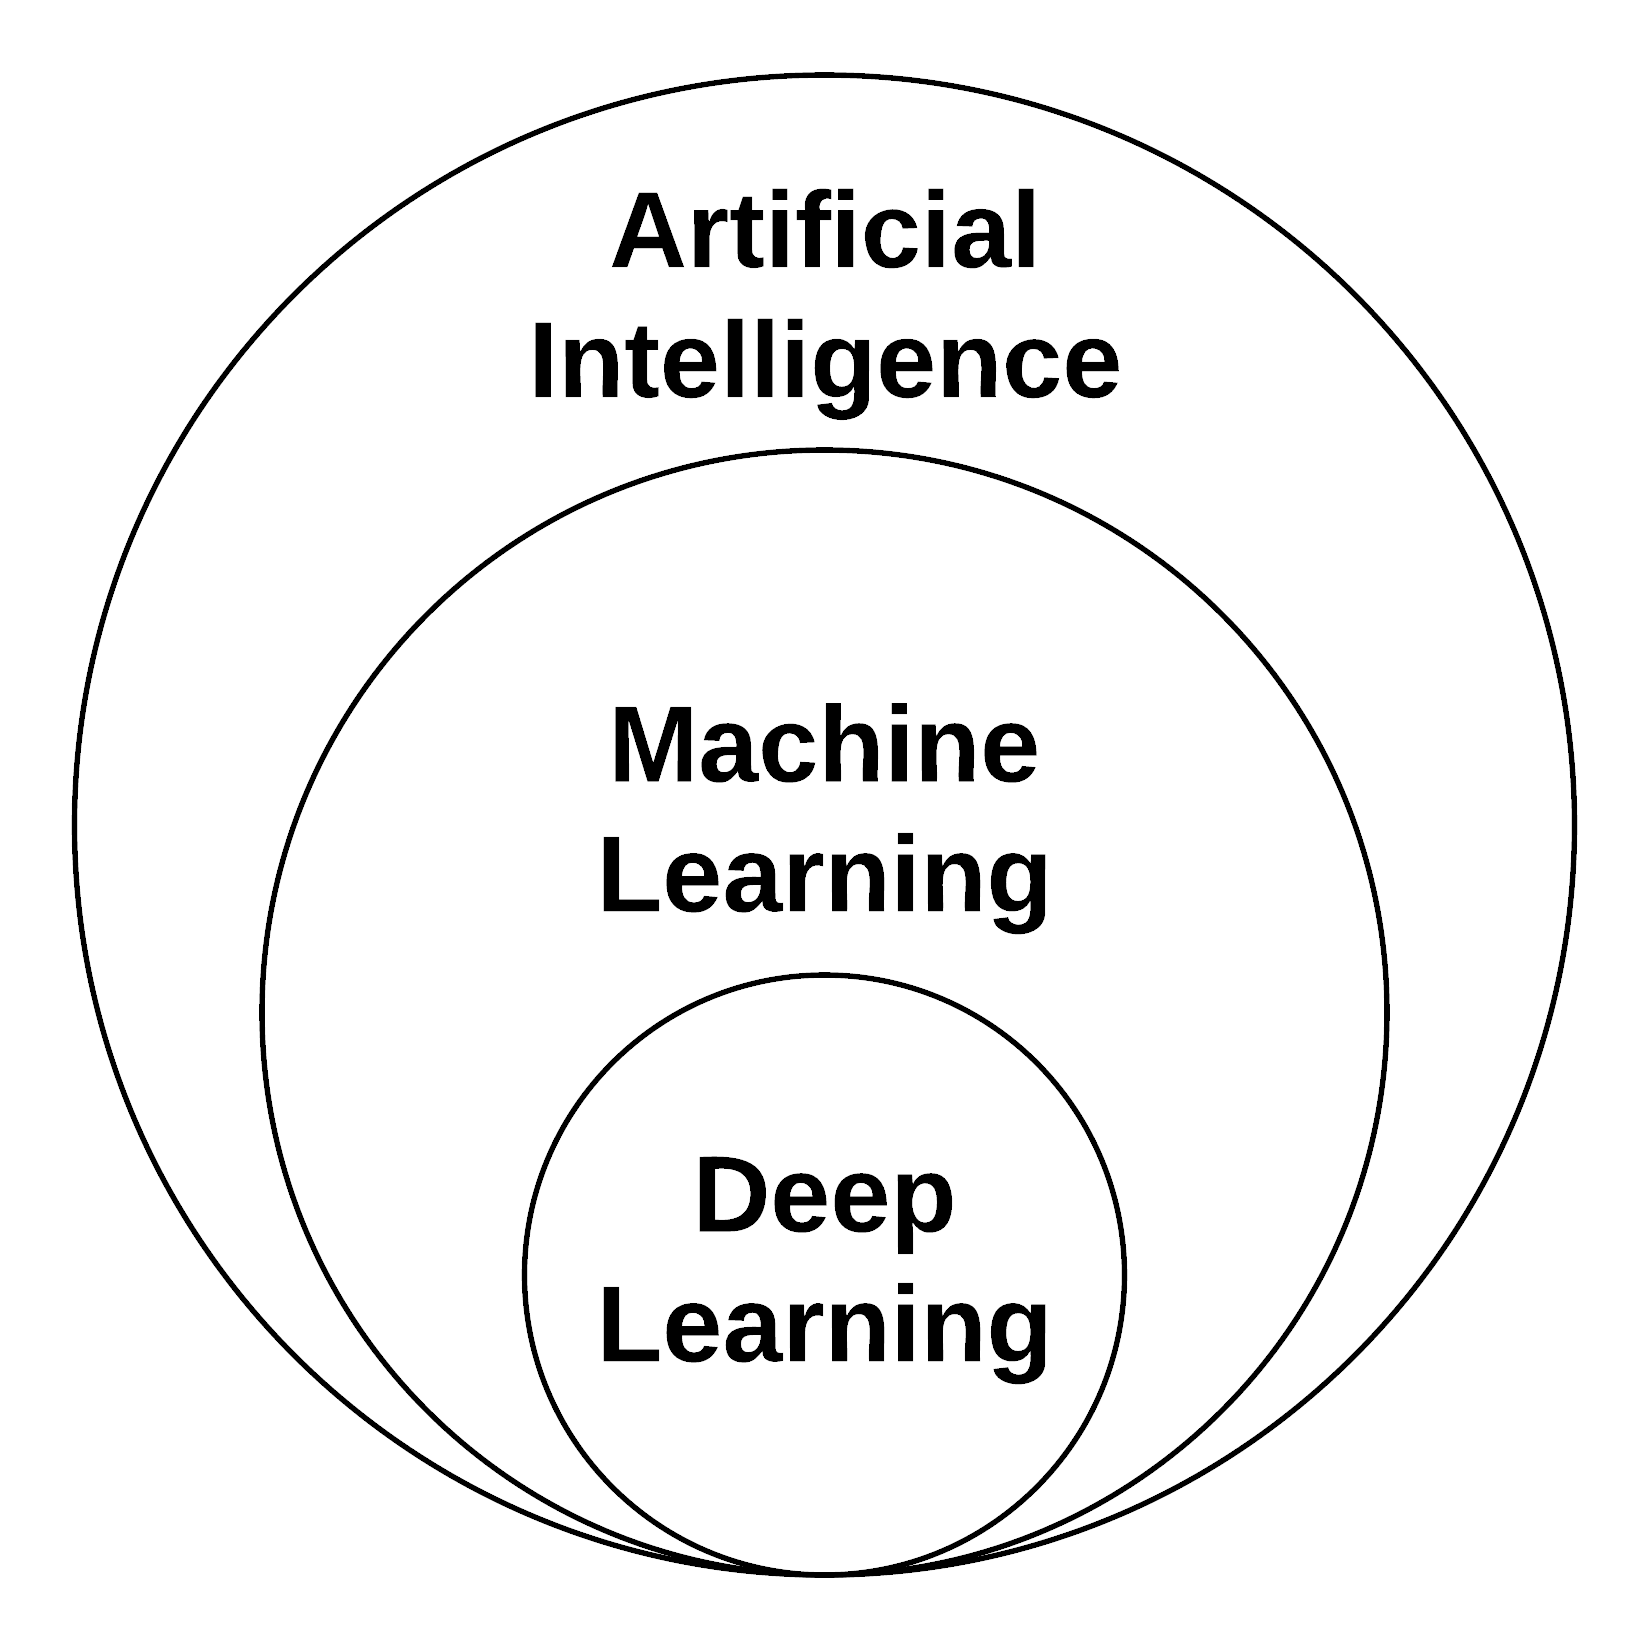
\includegraphics[width=0.3\textwidth]{figures/difference ml dl.png}
\end{wrapfigure}

\gls{dl} is a subfield of \gls{ml}, which is itself a subfield of \gls{ai}, as shown in Figure~\ref{fig:difference-ml-dl}. The main difference among each other is in the way algorithms learn. \gls{dl} algorithms automate most of the feature extraction from the data, whereas \gls{ml} relies more heavily on the experience of the person in charge of the feature engineering process.

The first \gls{ann} models were inspired by neurons and the brain's architecture, since nature has inspired many inventions throughout the history of humankind. This first model architecture was introduced by the neurophysiologist Warren McCulloch and the mathematician Walter Pitts~\cite{nnModelDefinition}.\newline

\subsection{Recurrent Neural Networks}

A \gls{rnn} looks very much like a feedforward \gls{ann}, except it also has connections pointing backward, Figure~\ref{fig:memory-cell}. Since the output of a recurrent neuron at time step t is a function of all the inputs from previous time steps, you could say it has a form of memory\cite{handsOnMachine}. This feature is extremely helpful when working with time related data such as stock prices.

\begin{figure}[H]
    \centering
    \caption{\label{fig:memory-cell} Memory cell}
    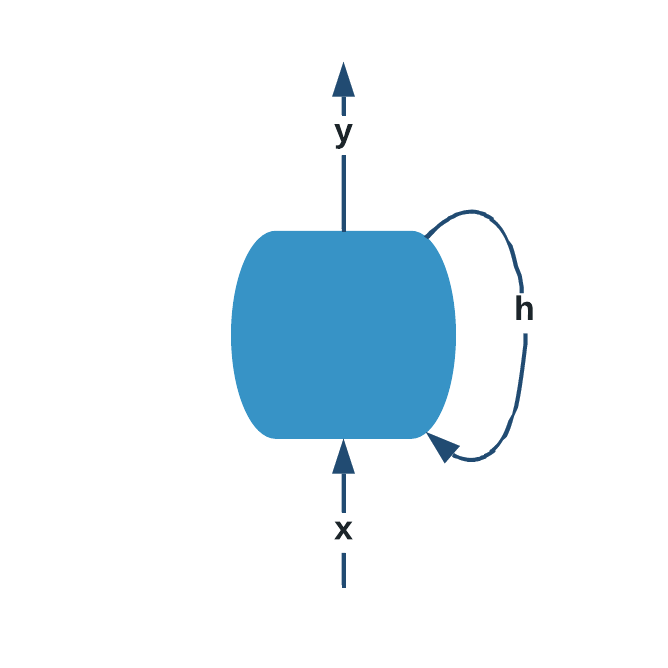
\includegraphics[width=0.30\textwidth]{figures/memory-cell.png}
\end{figure}

Due to the transformations that data undergo as it flows through an \gls{rnn}, some information is lost as time passes. After a while, the state contains practically no trace of the first entries. This phenomenon is called the vanishing gradient problem. The \gls{lstm} cell was proposed in 1997~\cite{lstm1997} by Sepp Hochreiter and Jürgen Schmidhuber and was explicitly designed to avoid the long-term dependency problem. Remembering information for long periods of time~\cite{understandLSTM}.

Although there are other approaches to deal with temporal data such as \glspl{cnn}, in this paper we will focus specifically on \gls{lstm} cells.

\section{Trading}

A trade could be defined as \enquote{the transfer of goods from one person or entity to another, often in exchange for money}~\cite{tradeDefinition}. This leads us to the natural concept of trading as an activity from which profits are expected when systematically applied. This behavior has been repeated throughout human history, as some studies show evidence of the exchange of obsidian and flint during the Stone Age~\cite{oxfordArcheology,obsidianTrade}. This phenomena can be seen as a starting point for modern economy.

Nonetheless, before further stepping into the concept of trading a clarification between the terms investing and trading is needed.

\subsection{Investing vs Trading}

Both terms are used interchangeably in a misleading manner, as they are two similar methods of attempting to make a profit~\cite{investingVsTrading}.

Investing takes a long-term approach where the goal is to gradually build wealth over a certain extended time frame by simply holding an asset the investor believes will appreciate over time, i.e., stocks, bonds, options, \glspl{etf} or real state, among others.

On the other hand, trading takes a completely different approach where the goal is to generate returns over short periods of time that outperforms holding investments by buying low and selling high. However, buying high and selling low is also a form of trading and is known as \gls{st}. There are four types of strategies depending on the period of time the trade is open for, as shown in Table~\ref{tab:types-trading}.

\begin{table}[h]
\caption{\label{tab:types-trading} Types of Trading}
\centering
\begin{tabular}{@{}|l|l|@{}}
    \toprule
    \multicolumn{1}{|c|}{\textbf{Trading Style}} & \multicolumn{1}{c|}{\textbf{Period of trade}} \\ \midrule
        Scalping         & Seconds/Minutes             \\
        Day Trading      & 1 Day                       \\
        Swing Trading    & Several days or even weeks  \\
        Position Trading & Weeks, months or even years \\ \bottomrule
\end{tabular}
\end{table}

\subsection{Machine learning applied to stock prediction}

Stock market forecasting is a fairly common topic in scientific and academic research, due to market's nature, and as mentioned previously, \gls{ml} algorithms are attracting a lot of attention in this matter due to the fact that \gls{ai} does pretty well dealing with pattern recognition. In addition to market patterns, many other macro factors can have an impact on the markets development, e.g, military conflicts, economic policies and even \textit{tweets}. All of which can be used by \gls{ai} algorithms to increase the accuracy in their predictions or decision making.

Both \gls{sl} and \gls{usl} algorithms have been used in stock market forecasting, but before steeping further into details we need a problem formulation for stock trading. "Considering the stochastic and interactive nature of the trading market, we can model it as a \gls{mdp}, which is specified as follows:"~\cite{practicalDeepLearningStock}

\begin{itemize}
    \item State \(s = [p, h, b] \): a set that includes the information of the prices of stocks p, the amount of holdings of stocks h and the remaining balance b.
    \item Action \(a\): a set of actions on all stocks. The available actions of each stock include selling, buying, and holding, which result in decreasing, increasing, and no change of the holdings h, respectively.
    \item Reward \(r(s, a, s')\): the change of the portfolio value when action a is taken at state \(s\) and arriving at the new state \(s'\).
    \item Policy \(\pi(s)\): the trading strategy of stocks at state \(s\). It is essentially the probability distribution of \(a\) at state \(s\).
    \item Action-value function \(Q\pi(s, a)\): the expected reward achieved by action \(a\) at state \(s\) following policy \(\pi\).
\end{itemize}

In their paper "Practical Deep Reinforcement Learning Approach for Stock Trading", Z. Xiong, X.-Y. Liu, S. Zhong, H. Yang y A. Walid\cite{practicalDeepLearningStock} use a \gls{ddpg} algorithm which is an improved version of the \gls{dpg} algorithm. As shown in Fig~\ref{fig:ddpg}, DDPG maintains an actor network and a critic network. The actor network \(\mu(s|\theta\mu\)) maps states to actions where \(\theta\mu\) is the set of actor network parameters, and the critic network \(Q(s, a|\theta Q)\) outputs the value of action under that state, where \(\theta Q\) is the set of critic network parameters. To explore better actions, a noise is added to the output of the actor network, which is sampled from a random process \(N\).~\cite{practicalDeepLearningStock} 

\begin{figure}[H]
    \centering
    \caption{\label{fig:ddpg} Learning Network Architecture~\cite{practicalDeepLearningStock}}
    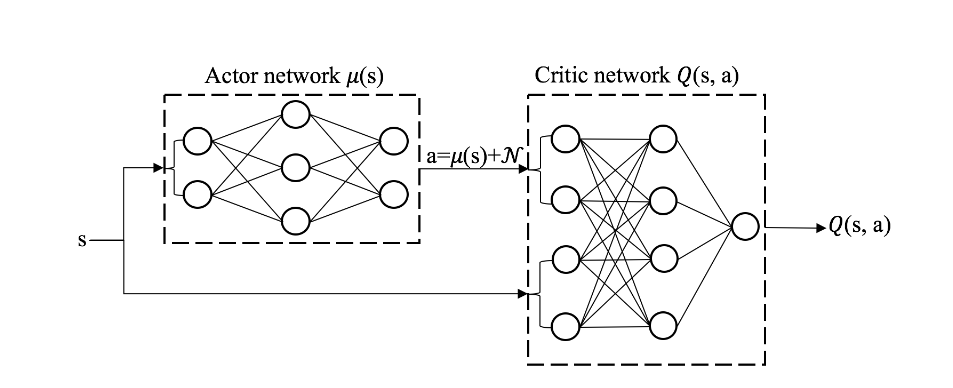
\includegraphics[width=0.85\textwidth]{figures/DDPG.png}
\end{figure}

\section{Containerization}

Over the last few years, there has been a paradigm shift in the computing field as on-premise hosted applications have gradually migrated to cloud based solutions. The concept of virtualization has played a key role in making this change possible given that some of the main advantages of cloud computing, i.e, resource efficiency, cost reduction and portability, are in part a result of virtualization technologies.

In this thesis we will talk about some different points of view of the containerization literature review. But before steeping further in, a clarifications between \gls{vm} and Container is needed.

\newpage
\subsection{Virtual Machine Vs Container}

\glspl{vm} and containers build on the same technologies and concepts. The main difference is that a \gls{vm} runs an entire \gls{os} instance on top of the \enquote{host} machine, whereas containers are intended for the deployment of single applications or services~\cite{containersStateOfArt}, as shown in Fig~\ref{fig:vm-container}

\begin{figure}[H]
    \centering
    \caption{\label{fig:vm-container} Virtual Machine vs Container, Source: www.netapp.com~\cite{vmVsContainer}}
    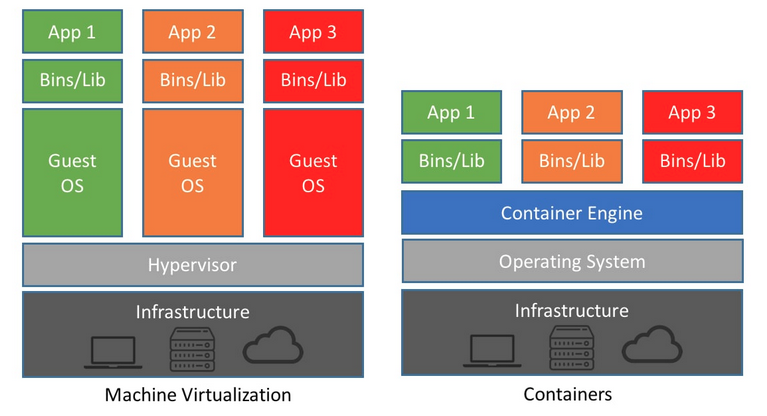
\includegraphics[width=0.65\textwidth]{figures/vm & container.png}
\end{figure}

\subsection{Orchestration}

In the container life cycle, orchestration supports automation and adaptation at run time. There are many challenges in this regard: design new processes and tools for performance monitoring, design resource and energy efficient auto scaling and scheduling algorithms and solutions for high availability. We will focus on auto scaling.

Among the auto scaling solutions, the most promising ones mix vertical and horizontal scaling and/or migration. Usually the auto scaling algorithms were designed for locally-distributed adaptation, but solutions that consider the geo-distributed case, suitable for \gls{iot} applications, have been
proposed as well. In high availability, the most promising approach is to make the detection of faulty nodes more sophisticated, e.g., based on abnormal behavior rather than only on network level or application level probes.~\cite{containersStateOfArt}

\subsection{Applications}

Containers offer an easy way to deploy Big data analytics applications based on the map-reduce or stream processing paradigms. Moreover, solutions are emerging to support the execution of containers on \gls{gpu} and \gls{fpga}, and to speedup specific analytic tasks.

Since containers are portable and have a small performance footprint, they are suitable to deploy applications on heterogeneous, resource and power limited computational units. Deploying containers on edge or fog computing nodes, or deploying containers on \gls{iot} boards like Rasperry
PI, is extremely advantageous, although it rises challenges in migration, service and resource provisioning and security.~\cite{containersStateOfArt}

\notebox{
    \textbf{\enquote{The SoTA in container technologies: Application, orchestration and security}}
    
    E. Casalicchio and S. Iannucci, provide a deep insight into different topics of containerization literature review. I strongly recommend reading their paper for those seeking a better understanding of the matter.
}

\section{Micro-services Architecture}
\label{Micro-services Architecture}

The only abstraction traditional programming languages such as C, Python or Java provide in terms of distribution and reduction of the complexity of programs is the breakdown of code into modules/packages. All of them produce single executable artifacts, also called monolith applications. Monolith applications are software programs whose modules can not be executed independently as Figure~\ref{fig:mono-app} shows. This feature generates several issues, among which:

\begin{itemize}
    \item Applications are difficult to maintain due to their larger complexity.
    \item Applications suffer from dependencies problems.
    \item Deployment processes are more complex.
    \item Scalability problems.
\end{itemize}

\begin{figure}[H]
    \centering
    \caption{\label{fig:mono-app}Monolithic Architecture, Source: www.n-ix.com~\cite{monoVsMicro}}
    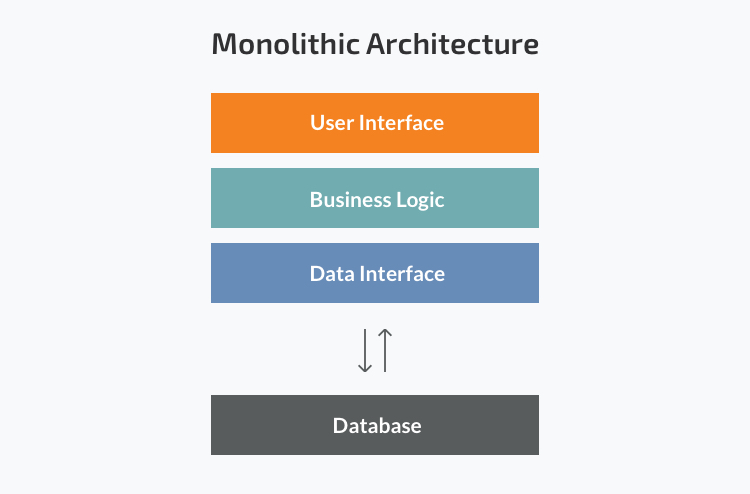
\includegraphics[width=0.5\textwidth]{figures/mono.jpg}
\end{figure}

\newpage
The micro-services architecture emerged as solution for these problems. It is in essence just a pattern that allows to decompose an application into smaller cohesive logical pieces called micro-services, mitigating most of the problems previously proposed Figure~\ref{fig:micro} . This smaller pieces communicate among each other through light messaging. Figure~\ref{fig:mono-vs-micro}

\begin{figure}[H]
    \centering
    \begin{subfigure}[a]{0.45\textwidth}
        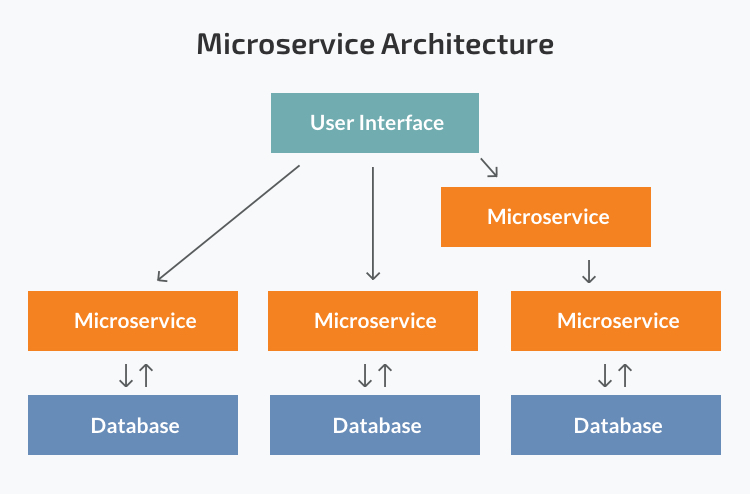
\includegraphics[width=\textwidth]{figures/micro.jpg}
        \caption{Micro-service architecture}
        \label{fig:micro}
    \end{subfigure}
    \hfill
    \begin{subfigure}[b]{0.54\textwidth}
        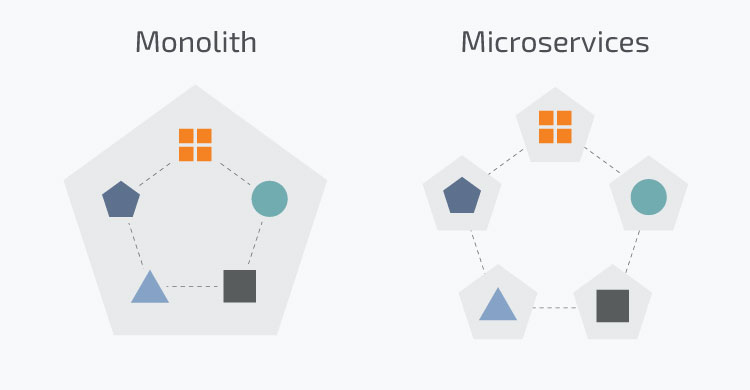
\includegraphics[width=\textwidth]{figures/micro vs mono.jpg}
        \caption{Monolith vs Micro-services}
        \label{fig:mono-vs-micro}
    \end{subfigure}
    \caption{\label{fig:mono-micro}Monolith vs Micro-services, Source: www.n-ix.com~\cite{monoVsMicro}}
\end{figure}

\subsection{Today}

According to~\cite{microservicesStateOfArt}, \enquote{Micro-services now are a new trend in software architecture, which emphasises the design and development of highly maintainable and scalable software. Micro-services manage growing complexity by functionally decomposing large systems into a set of independent services. By making services completely independent in development and deployment, micro-services emphasise loose coupling and high cohesion by taking modularity to the next level. This approach delivers all sorts of benefits in terms of maintainability, scalability, and so on.The micro-service architecture still shows distinctive characteristics that blend into something unique and different from \gls{soa} itself. The micro-service architecture gained popularity relatively recently and can be considered to be in its infancy since there is still a lack of consensus on what micro-services actually are}. Hence, micro-services offer a new modularity in software architecture that had not been practiced before and thus it has created a paradigm shift in this field of computation.

\subsection{Tomorrow}

According to~\cite{microservicesStateOfArt}, \enquote{The greatest strength of micro-services comes from pervasive distribution: even the internal components of software are autonomous services, leading to loosely coupled systems and the other benefits previously discussed. However, from this same aspect (distribution) also comes its greatest weakness: programming distributed systems is inherently harder than monoliths. We now have to think about new issues. Some examples are how can we manage changes to a service that may have side effects on other services that it communicates with? How can we prevent attacks that exploit network communications?. There are many pitfalls that we need to keep in mind when programming with micro services: a) Interfaces; b) Behavioural specifications and choreographies; c) Greater surface attack area; d) Network complexity; e) Trust.}
